Dopo aver introdotto le sfide di cybersecurity specifiche per le startup fintech, risulta fondamentale comprendere il contesto tecnologico in cui queste operano.
Attualmente, la stragrande maggioranza delle nuove imprese, specialmente nel settore tecnologico e finanziario, basa la propria infrastruttura su modelli di \textbf{cloud computing}.
Questo capitolo esplora i motivi di tale scelta, confrontando l'approccio cloud con quello tradizionale on-premises, e introduce \textbf{Amazon Web Services (AWS)}, il provider cloud prescelto per il nostro caso studio, delineandone la struttura e i principi fondamentali.

\section{Fondamenti di Cloud Computing}
Il \textit{cloud computing} (elaborazione tramite nuvola informatica) si configura come un modello di fruizione IT \textit{"on-demand"} che abilita l'accesso ubiquo e conveniente via rete a un pool condiviso di risorse computazionali configurabili (quali reti, server, storage, applicazioni e servizi), le quali possono essere predisposte o rilasciate rapidamente con il minimo sforzo di gestione o intervento da parte del provider \cite{nist800-145}.

Il modello di cloud computing definito dal \textit{National Institute of Standards and Technology (NIST)} si articola su cinque caratteristiche essenziali che ne delineano la natura e il funzionamento.
Queste caratteristiche sono cruciali per comprendere come il cloud si differenzi da altre forme tradizionali di gestione delle risorse IT e perché esso rappresenti un'evoluzione significativa per l'erogazione di servizi digitali.
Si analizzano di seguito tali caratteristiche in dettaglio:

\begin{itemize}
  \item \textbf{Autoservizio on-demand (On-demand self-service):} Gli utenti hanno la possibilità, in autonomia e senza l'intervento diretto del fornitore di servizi, di approvvigionarsi delle risorse di cui necessitano (come spazio di archiviazione, potenza di calcolo, ecc.) mediante interfacce self-service, spesso accessibili via web \cite{nist800-145}.

  \item \textbf{Accesso ampio alla rete (Broad network access):} Le risorse cloud sono accessibili attraverso la rete tramite meccanismi standard (ad esempio, browser web, applicazioni mobili), favorendo così l'utilizzo da dispositivi eterogenei quali smartphone, tablet, laptop e workstation \cite{nist800-145}.

  \item \textbf{Resource pooling (Multitenancy):} Le risorse del fornitore vengono raggruppate per servire più clienti (tenant) utilizzando un modello multi-tenant, in cui risorse fisiche e virtuali sono assegnate e riassegnate dinamicamente in base alla domanda dei vari utenti. Tale approccio garantisce efficienza e ottimizzazione nell'impiego dell'infrastruttura \cite{nist800-145}.

  \item \textbf{Rapid elasticity (Scalabilità rapida ed elasticità):} Le capacità possono essere scalate rapidamente, spesso in modo automatico, in base alle necessità dell'utente. Dal punto di vista del cliente, le risorse disponibili appaiono frequentemente illimitate e possono essere acquisite in qualsiasi quantità e in qualsiasi momento \cite{nist800-145}.

  \item \textbf{Servizio misurato (Measured service):} I sistemi cloud controllano e ottimizzano automaticamente l'uso delle risorse tramite capacità di misurazione appropriate (ad esempio, monitoraggio dell'archiviazione, dell'elaborazione, della larghezza di banda). Questo consente trasparenza sia per il provider sia per il consumatore del servizio \cite{nist800-145}.
\end{itemize}

\subsection{Modelli di servizio e distribuzione cloud}

I principali modelli di servizio e distribuzione cloud si rivelano fondamentali per l'innovazione e la crescita delle startup fintech. Essi permettono di accedere a risorse tecnologiche avanzate in modo flessibile e scalabile, spesso con una riduzione dei costi iniziali, accelerando l'innovazione e migliorando l'agilità operativa \cite{vats2024systematic, hrmars2025cloud}.
La comprensione di questi modelli è cruciale per le startup fintech che mirano a bilanciare efficienza, sicurezza e conformità normativa. Secondo lo standard internazionale ISO/IEC 17788, i modelli di servizio e di distribuzione offrono diverse opzioni per l'adozione del cloud \cite{iso2018overview}.

\subsubsection{Modelli di servizio cloud}

I modelli di servizio definiscono il livello di controllo e gestione dell'infrastruttura cloud da parte dell'utente. I tre modelli principali, \textit{Infrastructure as a Service (IaaS)}, \textit{Platform as a Service (PaaS)} e \textit{Software as a Service (SaaS)}, offrono diversi gradi di astrazione \cite{redhat2025cloud}.

\begin{figure}[htbp]
    \centering
    \includegraphics[width=0.9\textwidth]{cloud_service_models}
    \caption{Modelli di Servizio Cloud}
    \label{fig:service_models}
\end{figure}

\begin{itemize}
    \item \textbf{IaaS (Infrastructure as a Service):} questo modello fornisce infrastruttura IT on-demand, quali server, macchine virtuali, storage e rete, gestita dal provider cloud \cite{redhat2025cloud}. Le startup fintech possono così costruire e configurare ambienti IT complessi senza investire in hardware fisico, riducendo i costi di avvio e manutenzione \cite{vats2024systematic}. L'elasticità dell'IaaS consente di scalare rapidamente le risorse in base alla crescita del business o ai picchi di utilizzo, una caratteristica cruciale nel dinamico settore fintech \cite{vats2024systematic, hrmars2025cloud}.
    
    \item \textbf{PaaS (Platform as a Service):} questo modello fornisce una piattaforma completa, comprensiva di sistema operativo, middleware e strumenti di sviluppo, pronta per la creazione, l'esecuzione e la gestione di applicazioni \cite{redhat2025cloud}. Il provider gestisce l'infrastruttura sottostante, permettendo agli sviluppatori fintech di concentrarsi sull'innovazione del software \cite{vats2024systematic}. Ciò accelera il time-to-market di nuovi servizi finanziari e favorisce l'adozione di tecnologie avanzate come l'intelligenza artificiale e l'analisi dei dati \cite{vats2024systematic}.
    
    \item \textbf{SaaS (Software as a Service):} questo modello offre applicazioni software pronte all'uso accessibili tramite Internet, come sistemi di \textit{Customer Relationship Management (CRM)} o piattaforme di pagamento \cite{redhat2025cloud}. Le startup fintech possono integrare rapidamente soluzioni di terze parti nei propri processi, ottimizzando le risorse e focalizzandosi sull'esperienza utente e sull'innovazione dei servizi \cite{vats2024systematic}.
\end{itemize}

Questi modelli di servizio sono stati analizzati in studi sistematici e bibliometrici, i quali hanno evidenziato come la loro adozione, specialmente in contesti agili come le Piccole e Medie Imprese (PMI) e le startup fintech, apporti benefici in termini di flessibilità, riduzione dei costi e scalabilità \cite{vats2024systematic, hrmars2025cloud}.

\subsubsection{Modelli di distribuzione del cloud}

I modelli di distribuzione definiscono come l'infrastruttura cloud è resa disponibile e a chi è dedicata. I principali modelli includono il \textit{cloud pubblico (public cloud)}, il \textit{cloud privato (private cloud)}, il \textit{cloud ibrido (hybrid cloud)} e il \textit{cloud comunitario (community cloud)} \cite{maticmind2024hybrid, iso2018overview}.

\begin{itemize}
    \item \textbf{Public Cloud:} l'infrastruttura è di proprietà di un provider terzo (ad esempio, AWS, Azure, Google Cloud) e condivisa tra più clienti via Internet \cite{maticmind2024hybrid}. Per le startup fintech, il public cloud offre alta scalabilità e costi operativi proporzionali all'uso, risultando ideale per lanciare servizi senza investimenti iniziali significativi \cite{maticmind2024hybrid}. Tuttavia, la condivisione delle risorse può sollevare preoccupazioni per la sicurezza e il controllo diretto, aspetti critici per i dati finanziari \cite{vats2024systematic, maticmind2024hybrid}.
    
    \item \textbf{Private Cloud:} l'infrastruttura è dedicata a una singola organizzazione, garantendo livelli superiori di controllo, sicurezza e conformità normativa \cite{maticmind2024hybrid}. Questo aspetto è essenziale per le fintech che trattano dati sensibili. Lo svantaggio principale risiede nei costi più elevati e nella minore scalabilità immediata rispetto al cloud pubblico \cite{maticmind2024hybrid}.
    
    \item \textbf{Hybrid Cloud:} questo modello combina ambienti pubblici e privati, permettendo di spostare carichi di lavoro in base alle necessità \cite{maticmind2024hybrid}. Una startup fintech può utilizzare il public cloud per servizi meno critici e il private cloud per dati regolamentati, bilanciando flessibilità, scalabilità, sicurezza e compliance \cite{maticmind2024hybrid}. Tuttavia, l'adozione del cloud ibrido nel settore fintech presenta sfide di sicurezza specifiche, che possono essere mitigate, ad esempio, attraverso l'uso della tecnologia \textit{blockchain} (catena di blocchi) per garantire la compliance e la protezione dei dati sensibili \cite{urf2024security, vats2024systematic}. La gestione efficace di un ambiente ibrido è cruciale per ottimizzare i costi e mantenere la coerenza con i requisiti normativi \cite{maticmind2024hybrid}.
\end{itemize}

\subsection{Cloud Computing vs Infrastrutture On-Premises}
\label{sec:cloud-vs-onprem}

Tradizionalmente, le aziende gestivano la propria infrastruttura IT internamente, in data center di proprietà o in affitto. Questo modello è noto come \textbf{on-premises} (infrastruttura locale). Esso richiede l'acquisto di hardware (server, storage, apparati di rete), software (sistemi operativi, licenze) e l'impiego di personale specializzato per la gestione, la manutenzione, gli aggiornamenti e la sicurezza fisica ed operativa.

Il \textbf{cloud computing}, al contrario, si basa sull'erogazione di risorse informatiche (come potenza di calcolo, storage, database, reti, software, analytics, intelligenza artificiale) tramite Internet, secondo un modello \textit{pay-as-you-go} (pagamento basato sul consumo effettivo). I fornitori di servizi cloud, denominati \textit{Cloud Service Provider (CSP)}, come AWS, Microsoft Azure o Google Cloud Platform, gestiscono l'infrastruttura fisica sottostante, permettendo ai clienti di accedere alle risorse di cui hanno bisogno in modo flessibile e scalabile.

Le differenze principali risiedono nei seguenti aspetti:
\begin{itemize}
    \item \textbf{Costi:} L'approccio on-premises richiede un ingente investimento iniziale, noto come \textit{Capex (Capital Expenditure)}, per l'acquisto dell'hardware, mentre il cloud trasforma questo costo in una spesa operativa variabile, definita \textit{Opex (Operational Expenditure)}, basata sul consumo effettivo.
    \item \textbf{Scalabilità:} Il cloud offre una scalabilità \textit{elastica}, permettendo di aumentare o diminuire le risorse quasi istantaneamente in base alla domanda. L'infrastruttura on-premises presenta una scalabilità limitata e richiede pianificazione e acquisti anticipati per gestire picchi di carico.
    \item \textbf{Manutenzione:} Nel cloud, la manutenzione dell'hardware e dell'infrastruttura di base è responsabilità del provider, liberando il team IT del cliente da tali incombenze.
    \item \textbf{Agilità e Velocità:} Il cloud permette di predisporre nuove risorse in pochi minuti, accelerando notevolmente i cicli di sviluppo e il \textit{time-to-market} (tempo di immissione sul mercato) di nuovi prodotti o servizi.
    \item \textbf{Affidabilità e Portata Globale:} I principali CSP dispongono di data center ridondati in diverse regioni geografiche, offrendo alta disponibilità e la possibilità di distribuire applicazioni a livello globale con bassa latenza.
\end{itemize}

\subsection{Perché le Startup Scelgono il Cloud}
\label{sec:startup-cloud-choice}

Per le startup, e in modo particolarmente accentuato per quelle operanti nel dinamico settore fintech che richiedono elevata agilità e una gestione efficiente delle risorse, il modello cloud computing offre vantaggi strategici e operativi decisivi rispetto alle tradizionali infrastrutture on-premises. Tali vantaggi includono:

\begin{itemize}
\item \textbf{Riduzione delle Barriere all'Ingresso e Ottimizzazione dei Costi:} L'eliminazione di ingenti investimenti iniziali in hardware e software (Capex) rende accessibili tecnologie avanzate anche a entità con budget limitati. Il modello di pagamento basato sul consumo effettivo (Opex) permette di allineare i costi direttamente alla crescita e all'utilizzo reale delle risorse.
\item \textbf{Agilità e Adattabilità delle Risorse:} Le startup possono avviare le proprie operazioni con un dimensionamento infrastrutturale minimo, per poi espandere o contrarre rapidamente le risorse in risposta alle dinamiche del mercato o alla crescita della base utenti e del volume transazionale. Questa capacità è fondamentale nel fintech, dove la domanda può essere volatile e imprevedibile. Le modalità tecniche attraverso cui si realizza tale agilità, ovvero scalabilità ed elasticità, saranno analizzate in dettaglio nel prosieguo della sezione.
\item \textbf{Focalizzazione Strategica sul Core Business:} Delegando la gestione, la manutenzione e l'aggiornamento dell'infrastruttura IT al Cloud Service Provider (CSP), la startup può concentrare le proprie risorse umane e finanziarie, spesso limitate, sullo sviluppo del prodotto, sull'innovazione di servizio e sull'acquisizione di quote di mercato, piuttosto che sulla complessa gestione dei sistemi.
\item \textbf{Accelerazione del Time-to-Market:} La capacità di predisporre e de-predisporre rapidamente ambienti di sviluppo, test e produzione consente di abbreviare significativamente i cicli di rilascio di nuove funzionalità e servizi, un fattore competitivo critico in settori ad alta innovazione come il fintech.
\item \textbf{Accesso a Tecnologie Avanzate e Servizi Gestiti:} I CSP mettono a disposizione un vasto portafoglio di servizi all'avanguardia, pronti all'uso e gestiti, che includono database performanti, piattaforme di machine learning, strumenti di big data analytics e soluzioni di sicurezza. L'implementazione e la gestione autonoma di tali tecnologie on-premises comporterebbero costi e complessità proibitivi per la maggior parte delle startup.
\item \textbf{Elevati Livelli di Resilienza, Disponibilità e Sicurezza Infrastrutturale:} I CSP investono massicciamente in infrastrutture ridondanti e geograficamente distribuite, offrendo elevati livelli di disponibilità (tipicamente garantiti da \textit{Service Level Agreement - SLA}, accordi sul livello di servizio) e resilienza operativa, spesso superiori a quanto una startup potrebbe garantire autonomamente. Questo si combina con solide fondamenta di sicurezza fisica e operativa dei data center (sebbene la sicurezza nel cloud, relativa ai dati e alle applicazioni, rimanga una responsabilità condivisa e primariamente del cliente).
\end{itemize}

Questi vantaggi traggono origine, a livello infrastrutturale, da caratteristiche intrinseche dei modelli cloud che risultano particolarmente sinergiche con le esigenze del fintech. Tra queste, spiccano la scalabilità, la flessibilità e l'elasticità, le cui specificità verranno ora analizzate.

\textbf{Scalabilità (Scalability):} Si riferisce alla capacità intrinseca di un sistema di incrementare la propria capacità elaborativa e di gestione dei dati per far fronte a un aumento del carico di lavoro. Tale incremento può essere pianificato (ad esempio, in previsione di una crescita organica del numero di utenti o di transazioni) e si attua mediante l'aggiunta di risorse (\textit{scale-out}, aggiungendo più nodi) o l'aumento della potenza dei nodi esistenti (\textit{scale-up}, incrementando le risorse di un singolo nodo). Per una startup fintech, la scalabilità assicura che l'infrastruttura possa supportare l'espansione del business e gestire volumi di domanda crescenti, anche se caratterizzati da ciclicità prevedibile (ad esempio, picchi di fine mese per elaborazione stipendi o rendicontazioni).

\textbf{Flessibilità (Flexibility):} Concerne la possibilità di scegliere, configurare e modificare un'ampia gamma di risorse, servizi e modelli operativi offerti dalla piattaforma cloud. Include la facoltà di selezionare diverse tipologie di istanze computazionali, opzioni di storage, database, servizi di intelligenza artificiale, strumenti di networking e sicurezza. Per una startup fintech, la flessibilità si traduce nella capacità di sperimentare rapidamente nuove soluzioni, integrare servizi di terze parti, adattarsi a requisiti normativi mutevoli o modificare l'architettura applicativa senza vincoli infrastrutturali stringenti. Oltre alla vasta gamma di opzioni tecnologiche, la flessibilità si estende ai modelli contrattuali e di pricing (ad esempio, istanze on-demand, reserved instances, spot instances), consentendo un'ulteriore ottimizzazione dei costi in base a profili di utilizzo specifici e alla strategia finanziaria della startup.

\textbf{Elasticità (Elasticity):} Rappresenta una forma dinamica e, idealmente, automatizzata di scalabilità. L'elasticità permette al sistema di allocare e deallocare risorse computazionali (come capacità di calcolo, memoria o banda) in maniera automatica e in tempo reale, in risposta a fluttuazioni immediate e spesso imprevedibili del carico di lavoro \cite{cloudsurvey2019}. A differenza della scalabilità, che può implicare interventi pianificati, l'elasticità reagisce autonomamente a picchi improvvisi (\textit{burst}) o a cali repentini della domanda, ottimizzando sia le prestazioni che i costi.

La sinergia di queste tre caratteristiche – scalabilità, flessibilità ed elasticità – consente alle startup fintech di ottimizzare l'allocazione dei costi infrastrutturali, aderendo pienamente al principio del "pay-per-use" (pagamento basato sull'effettivo consumo), e di garantire livelli prestazionali adeguati e resilienti. Questa sinergia è particolarmente vitale per le startup fintech, che operano in un mercato caratterizzato da un'intensa competizione, una rapida evoluzione delle aspettative dei consumatori e una continua innovazione tecnologica, richiedendo la massima reattività e capacità di adattamento per mantenere e incrementare la propria competitività.

\subsection{Introduzione ad Amazon Web Services (AWS)}
\label{sec:aws-intro}

Tra i principali fornitori di servizi cloud, \textbf{Amazon Web Services (AWS)} si posiziona come leader di mercato e rappresenta la scelta infrastrutturale per moltissime startup a livello globale, incluse quelle operanti nel settore fintech, come nel caso studio di questa tesi. Lanciato nel 2006, AWS offre un portafoglio estremamente ampio e maturo di servizi cloud.

La struttura di AWS si basa su alcuni concetti chiave:

\begin{itemize}
    \item \textbf{Infrastruttura Globale:} AWS opera attraverso una rete mondiale di \textbf{Regioni}. Ogni Regione è un'area geografica fisica separata (ad esempio, Irlanda, Francoforte, Nord Virginia). All'interno di ciascuna Regione, esistono multiple \textbf{Zone di Disponibilità (Availability Zones - AZ)}. Una AZ è costituita da uno o più data center discreti, con alimentazione, raffreddamento e rete ridondati. Le AZ all'interno di una Regione sono interconnesse con reti a bassa latenza ma sono fisicamente separate per garantire l'isolamento in caso di guasti (come incendi o allagamenti). Questa architettura permette di costruire applicazioni altamente disponibili e tolleranti ai guasti, distribuendole su più AZ.
    \item \textbf{Servizi Fondamentali:} AWS offre centinaia di servizi, ma alcuni sono considerati fondamentali:
        \begin{itemize}
            \item \textbf{Compute:} Servizi per l'esecuzione di codice, come \textit{Amazon Elastic Compute Cloud (Amazon EC2)} per macchine virtuali scalabili, \textit{AWS Lambda} per l'esecuzione di codice serverless (senza la gestione di server), e servizi container come \textit{Amazon Elastic Container Service (ECS)} ed \textit{Amazon Elastic Kubernetes Service (EKS)}.
            \item \textbf{Storage:} Servizi per l'archiviazione dei dati, come \textit{Amazon Simple Storage Service (Amazon S3)} per lo storage a oggetti altamente duraturo e scalabile, \textit{Amazon Elastic Block Store (Amazon EBS)} per volumi a blocchi destinati alle istanze EC2, e \textit{Amazon Elastic File System (Amazon EFS)} per file system condivisi.
            \item \textbf{Database:} Una vasta gamma di database gestiti, inclusi database relazionali (\textit{Amazon Relational Database Service - Amazon RDS}), NoSQL (\textit{Amazon DynamoDB}), data warehouse (\textit{Amazon Redshift}), ecc.
            \item \textbf{Networking:} Servizi per definire e controllare la rete virtuale, come \textit{Amazon Virtual Private Cloud (Amazon VPC)} per creare reti isolate, \textit{Elastic Load Balancing (ELB)} per distribuire il traffico, e \textit{AWS Direct Connect} per connessioni dedicate.
            \item \textbf{Security, Identity, \& Compliance:} Servizi per gestire accessi, sicurezza e conformità, come \textit{AWS Identity and Access Management (IAM)}, \textit{AWS Key Management Service (KMS)}, \textit{AWS Web Application Firewall (WAF)}, \textit{Amazon GuardDuty} (per il rilevamento delle minacce).
        \end{itemize}
    \item \textbf{Modello Pay-as-you-go:} Come accennato, si paga solo per le risorse effettivamente consumate, senza contratti a lungo termine o costi iniziali (per la maggior parte dei servizi).
    \item \textbf{Modello di Responsabilità Condivisa (Shared Responsibility Model)}: È cruciale comprendere che la sicurezza su AWS è una responsabilità condivisa. AWS è responsabile della sicurezza *del* cloud (l'infrastruttura fisica, la rete, l'hypervisor), mentre il cliente è responsabile della sicurezza *nel* cloud (la configurazione dei servizi, la gestione degli accessi, la protezione dei dati, la sicurezza del sistema operativo e delle applicazioni).
\end{itemize}

\subsection{Il Caso Specifico: AWS per la Startup fintech}
\label{sec:aws-for-fintech}

La selezione di AWS quale infrastruttura cloud per la startup fintech oggetto di questa tesi è il risultato di una valutazione strategica, basata su fattori tecnici e di business specifici. Oltre ai benefici generali offerti dal cloud computing, AWS presenta caratteristiche particolarmente determinanti per un operatore del settore finanziario:
\begin{itemize}
    \item \textbf{Maturità e Affidabilità:} Essendo il provider cloud più longevo e con la più vasta quota di mercato, AWS vanta una comprovata esperienza nella gestione di carichi di lavoro \textit{mission-critical} (critici per la missione aziendale). Tale affidabilità è essenziale per un settore, come quello finanziario, che richiede massima operatività e fiducia da parte degli utenti.
    \item \textbf{Ampiezza dei Servizi:} Il vasto portafoglio di servizi AWS permette di costruire architetture complesse, resilienti e moderne. Esso consente di integrare nativamente servizi per l'analisi avanzata dei dati, il machine learning (fondamentale, ad esempio, per sistemi antifrode, credit scoring o personalizzazione dei servizi finanziari), e la gestione sicura delle transazioni.
    \item \textbf{Supporto alla Compliance:} AWS offre documentazione dettagliata, strumenti e servizi specifici (come AWS Artifact per l'accesso ai report di compliance) che aiutano le organizzazioni a soddisfare i rigorosi standard di conformità richiesti nel settore finanziario, tra cui PCI DSS, GDPR, ISO 27001 e normative locali specifiche. AWS stessa mantiene numerose certificazioni internazionali per la propria infrastruttura, fornendo una base solida su cui costruire applicazioni conformi.
    \item \textbf{Scalabilità e Performance Elevate:} La capacità di scalare le risorse in modo elastico e di garantire alte prestazioni è fondamentale per gestire picchi transazionali improvvisi (ad esempio, durante l'apertura dei mercati o in seguito a campagne promozionali) e assicurare tempi di risposta rapidi, critici per l'esperienza utente nei servizi finanziari.
    \item \textbf{Ecosistema di Partner Specializzati:} Esiste un vasto ecosistema di partner tecnologici e di consulenza con competenze specifiche su AWS, inclusi numerosi attori con expertise verticale nel settore fintech, in grado di supportare la startup in fasi di progettazione, implementazione e gestione.
    \item \textbf{Servizi di Sicurezza Avanzati e Stratificati:} AWS offre un set robusto e profondo di strumenti nativi per implementare controlli di sicurezza a molteplici livelli (rete, identità, dati, rilevamento delle minacce, crittografia), aspetti che verranno analizzati in dettaglio nei capitoli successivi.
\end{itemize}
Nei capitoli successivi, si analizzerà in dettaglio come l'infrastruttura di questa specifica startup fintech sia stata progettata e messa in sicurezza sfruttando i servizi e le \textit{best practice} (migliori pratiche) offerte da AWS, con un focus sulle implicazioni e le scelte architetturali per un operatore del settore finanziario.

\subsection{Infrastruttura Globale AWS: Fondamenta per la fintech}
\label{sec:aws-global-infra-fintech}

Amazon Web Services (AWS) dispone di una infrastruttura globale altamente distribuita: nel 2025 il cloud AWS è esteso su 36 Regioni geografiche (ciascuna costituita da più Availability Zone) per un totale di 114 Availability Zones lanciate \cite{aws-global-infra}. Ogni Regione AWS rappresenta un'area geografica distinta, fisicamente isolata dalle altre per garantire \textit{fault tolerance} (tolleranza ai guasti) e permettere il rispetto dei requisiti regolamentari sulla sovranità dei dati \cite{aws-global-infra}. All'interno di ogni Regione sono presenti almeno tre \textit{Availability Zone (AZ)}, concepite come data center indipendenti dal punto di vista dell'alimentazione, del raffreddamento e della connettività di rete fisica, pur essendo interconnesse tramite collegamenti privati ridondanti ad alta velocità e bassa latenza \cite{aws-global-infra}.

Questo design multi-AZ è particolarmente critico per una startup fintech: la capacità di resistere a guasti localizzati (come un'interruzione di corrente in un data center o un evento catastrofico limitato a una singola AZ) senza interruzione del servizio è fondamentale per mantenere la continuità operativa nelle transazioni finanziarie, preservare la fiducia degli utenti e rispettare potenziali requisiti normativi sulla disponibilità dei servizi. Secondo AWS, ciò garantisce un'elevata disponibilità dell'infrastruttura e contiene l'impatto di eventuali interruzioni all'interno della Regione interessata \cite{aws-global-infra}.

Per supportare applicazioni globali a bassa latenza, cruciali per l'esperienza utente nei servizi finanziari digitali, AWS integra inoltre le \textit{Edge Location} (punti di presenza perimetrali) e le \textit{Local Zone} (zone locali). Le Edge Location (oltre 700 nel mondo) sono data center che ospitano servizi come Amazon CloudFront, una \textit{Content Delivery Network (CDN)} (rete per la consegna di contenuti) che permette la consegna rapida di contenuti statici e dinamici agli utenti finali. CloudFront instrada le richieste al \textit{punto di presenza (PoP)} geograficamente più vicino all'utente, minimizzando la latenza \cite{aws-cloudfront}. Le Local Zone sono estensioni dell'infrastruttura AWS posizionate strategicamente vicino a grandi centri urbani o industriali, progettate per offrire latenze nell'ordine dei millisecondi a singola cifra per scenari applicativi specifici (ad esempio, sistemi di trading ad alta frequenza, elaborazione di pagamenti in tempo reale o applicazioni di realtà aumentata per servizi finanziari).

Il backbone di rete globale AWS, basato su una dorsale in fibra ottica ridondata che interconnette le Regioni con capacità fino a 400 Gb/s \cite{aws-network}, è un altro asset fondamentale. Tutti i dati che transitano su questa rete globale tra i data center e le Regioni AWS vengono crittografati automaticamente a livello fisico prima di lasciare le strutture protette \cite{aws-network}. Il cliente, inoltre, mantiene il pieno controllo sui propri dati, inclusa la facoltà di applicare ulteriori livelli di crittografia utilizzando servizi dedicati. Questa solida infrastruttura di rete non solo garantisce performance elevate, ma la crittografia automatica dei dati in transito aggiunge un livello di sicurezza fondamentale per i dati finanziari sensibili.

Dal punto di vista di una startup fintech, una siffatta infrastruttura globale distribuita offre vantaggi tangibili. La possibilità di collocare geograficamente le risorse permette di posizionare le applicazioni e i dati vicino agli utenti finali o in specifiche giurisdizioni per soddisfare requisiti di bassa latenza (cruciali per l'esperienza utente in app finanziarie) e di sovranità dei dati (come il GDPR). L'ampia rete backbone e la sua crittografia intrinseca proteggono le comunicazioni inter-regionali, essenziali ad esempio per strategie di disaster recovery. Le Edge Location, tramite CloudFront, possono accelerare significativamente l'erogazione di interfacce web o API rivolte ai clienti, migliorando la reattività delle piattaforme fintech, un fattore competitivo chiave.

\subsection{Architettura Virtualizzata e Meccanismi di Scalabilità per la fintech}
\label{sec:virtualization-scalability-fintech}

Le risorse computazionali su AWS sono erogate principalmente attraverso tecnologie di \textit{virtualizzazione}. Su ogni server fisico (host) viene eseguito un \textit{hypervisor} (monitor di macchine virtuali), un software che astrae l'hardware sottostante e crea molteplici istanze virtuali isolate tra loro. In AWS, la virtualizzazione, storicamente basata su hypervisor Xen e più recentemente sul sistema AWS Nitro (che include un hypervisor leggero basato su KVM, Kernel-based Virtual Machine) \cite{aws-nitro-hypervisor}, consente di eseguire su un singolo server fisico decine di \textit{macchine virtuali (VM)} indipendenti, ciascuna con il proprio sistema operativo e le proprie applicazioni \cite{ibm_iaas}. L'hypervisor assegna a ogni VM una porzione dedicata di CPU, memoria e storage, garantendo l'isolamento delle risorse e della sicurezza tra le istanze \cite{ibm_iaas}.

Grazie alla virtualizzazione, più tenant (clienti AWS) possono condividere in modo sicuro lo stesso hardware fisico sottostante; questo è il concetto di \textit{multitenancy} (multi-locazione), definito dal NIST come un'architettura in cui "una singola istanza di un software gira su un server ed è usata da più tenant" \cite{nist800-145}. In pratica, anche in un modello multitenant come quello di AWS, ogni cliente opera all'interno del proprio ambiente virtuale logicamente isolato, con i propri dati segregati, grazie a meccanismi di isolamento di rete (ad esempio, \textit{Virtual Private Cloud - VPC}) e alle garanzie fornite dal software di virtualizzazione. Per una startup fintech, il modello multitenant, pur offrendo significativi vantaggi in termini di costi e agilità, richiede un'attenta valutazione e l'implementazione di robuste strategie di isolamento a livello applicativo e di rete, complementari a quelle fornite da AWS, per garantire la segregazione e la protezione dei dati finanziari sensibili.

La virtualizzazione è il fulcro dell'offerta IaaS di AWS. Come delineato nel modello di responsabilità condivisa (descritto in seguito), AWS gestisce l'infrastruttura fisica sottostante (hardware, networking, data center, patching dell'hypervisor), mentre il cliente mantiene il controllo sul sistema operativo guest, sugli aggiornamenti software, sulle configurazioni di sicurezza dell'ambiente virtuale e sulle applicazioni \cite{aws-well-architected}. Ad esempio, quando si avvia un'istanza Amazon EC2 (il servizio IaaS di AWS), AWS fornisce la macchina virtuale, ma è responsabilità del cliente gestirne il sistema operativo, le patch di sicurezza e il software applicativo. Questa astrazione permette di orchestrare e scalare migliaia di istanze virtuali con un elevato grado di automazione.

Per gestire la crescita del carico di lavoro e le fluttuazioni della domanda, tipiche del settore fintech, AWS offre due principali meccanismi di scalabilità:
\begin{itemize}
    \item La \textbf{scalabilità verticale} (scale-up) consiste nell'aumentare le risorse di una singola istanza (ad esempio, incrementando CPU, RAM o capacità di I/O del disco) \cite{awsAutoScaling}. Questa strategia può essere utile per carichi di lavoro monolitici o database, ma presenta limiti fisici intrinseci e può introdurre un \textit{single point of failure} (singolo punto di guasto) se non gestita con ridondanza. Per una startup, può essere una soluzione iniziale, ma la sua limitata resilienza la rende meno adatta per carichi di lavoro critici nel settore fintech a lungo termine.
    \item La \textbf{scalabilità orizzontale} (scale-out) implica la distribuzione del carico di lavoro su più istanze o nodi, replicando l'applicazione \cite{awsAutoScaling}. Ad esempio, si possono avviare più istanze EC2 identiche dietro un bilanciatore di carico (come Elastic Load Balancing). In questo modo, il traffico utente viene distribuito tra le VM disponibili, e il sistema può tollerare il guasto di singole istanze senza interrompere il servizio. La scalabilità orizzontale è particolarmente vantaggiosa per le applicazioni fintech, che spesso sperimentano fluttuazioni significative nel carico di lavoro (ad esempio, durante l'apertura dei mercati, eventi promozionali, o picchi di fine mese per elaborazioni contabili). La capacità di aggiungere o rimuovere istanze dinamicamente, spesso gestita da servizi come AWS Auto Scaling \cite{awsAutoScaling}, permette alla startup di mantenere performance ottimali e controllare i costi in modo efficiente, pagando solo per le risorse effettivamente utilizzate.
\end{itemize}

Per massimizzare la disponibilità delle applicazioni, un requisito non negoziabile per i servizi finanziari, in AWS si progetta attivamente per la resilienza utilizzando repliche \textit{multi-AZ} (distribuite su più Zone di Disponibilità). Ad esempio, il servizio Amazon RDS consente di creare istanze database in configurazione Multi-AZ: quando questa opzione è abilitata, AWS provvede automaticamente a creare e mantenere una replica sincrona (standby) del database primario in una Availability Zone differente all'interno della stessa Regione \cite{aws-rds-multiaz}. Tutte le modifiche al database primario vengono replicate in tempo reale alla standby. In caso di guasto dell'istanza primaria o dell'intera AZ in cui risiede, RDS gestisce un \textit{failover} (passaggio automatico alla replica) trasparente alla replica standby, minimizzando i tempi di indisponibilità, noti come \textit{Recovery Time Objective (RTO)}. Questa funzionalità è di importanza critica per una startup fintech, poiché la perdita di accesso al database transazionale principale potrebbe comportare l'interruzione dei servizi, perdite finanziarie e danni reputazionali significativi. Analogamente, servizi come Elastic Load Balancing possono e devono essere configurati per distribuire il traffico su istanze dislocate in multiple AZ, garantendo che un'interruzione locale sia compensata dagli altri nodi attivi. Le scelte architetturali per l'alta disponibilità includono quindi l'uso sistematico di configurazioni multi-AZ, il bilanciamento del carico e la replica dei dati (eventualmente su più Regioni per il \textit{disaster recovery}, recupero da disastro).

Nei casi estremi di disastro che potrebbero compromettere un'intera Regione AWS, è necessario implementare strategie di Disaster Recovery (DR) più complesse, come delineato nel Well-Architected Framework di AWS \cite{awsWellArchitected}. Tra queste strategie si annoverano:
\begin{itemize}
    \item \textbf{Backup and Restore (Backup e Ripristino):} Utilizzo di snapshot periodici dei dati (ad esempio, archiviati su Amazon S3 e Amazon S3 Glacier) e template infrastrutturali (ad esempio, AWS CloudFormation) per ricreare l'infrastruttura e ripristinare i dati in una Regione secondaria. È la strategia con RTO e \textit{Recovery Point Objective (RPO)} (obiettivo del punto di ripristino, ovvero la massima perdita di dati accettabile) più elevati.
    \item \textbf{Pilot Light (Fiamma Pilota):} Mantenimento di una copia minima dell'infrastruttura (core infrastrutturale) e dei dati critici costantemente replicati nella Regione di DR. Le risorse applicative principali vengono attivate solo in caso di disastro.
    \item \textbf{Warm Standby (Standby Tiepido):} Mantenimento di una versione scalata ridotta, ma pienamente funzionante, dell'applicazione nella Regione di DR, pronta a gestire il traffico in caso di failover.
    \item \textbf{Multi-site Active/Active (o Hot Standby, Standby Caldo):} L'applicazione è dispiegata e attivamente serve traffico contemporaneamente in due o più Regioni, con meccanismi di bilanciamento del carico geografico. È la strategia più complessa e costosa, ma offre l'RTO e l'RPO più bassi.
\end{itemize}
La scelta della strategia di DR per una startup fintech dipenderà da una valutazione del rischio, dai requisiti normativi (spesso stringenti nel settore finanziario per quanto riguarda la continuità operativa e i tempi di ripristino) e dal budget disponibile. AWS fornisce strumenti come AWS Resilience Hub \cite{aws-resilience} per aiutare a definire, testare e monitorare la postura di resilienza delle applicazioni, assicurando che i tempi di recovery (RTO) e la perdita massima di dati accettabile (RPO) siano allineati con le esigenze di business e i requisiti di compliance.

\subsection{Modello di Responsabilità Condivisa: Implicazioni per la fintech}
\label{sec:shared-responsibility-fintech}

La sicurezza nel cloud AWS opera secondo il \textit{modello di responsabilità condivisa} (\textit{Shared Responsibility Model}) \cite{aws-shared-responsibility}. Questo modello distingue nettamente le responsabilità di AWS da quelle del cliente. In sintesi, AWS è responsabile della \textit{sicurezza "del" cloud ("security of the cloud")}. Ciò include la protezione dell'infrastruttura fisica e globale che esegue tutti i servizi AWS: l'hardware, il software di base (hypervisor, sistemi operativi dei servizi gestiti), la rete e le strutture fisiche (data center), compresi i controlli fisici e ambientali. AWS investe significativamente in misure quali sorveglianza 24/7, rigorosi controlli degli accessi fisici alle strutture, ridondanza dei sistemi e patching dell'infrastruttura sottostante \cite{aws-shared-responsibility}.

\begin{figure}[htbp]
    \centering
    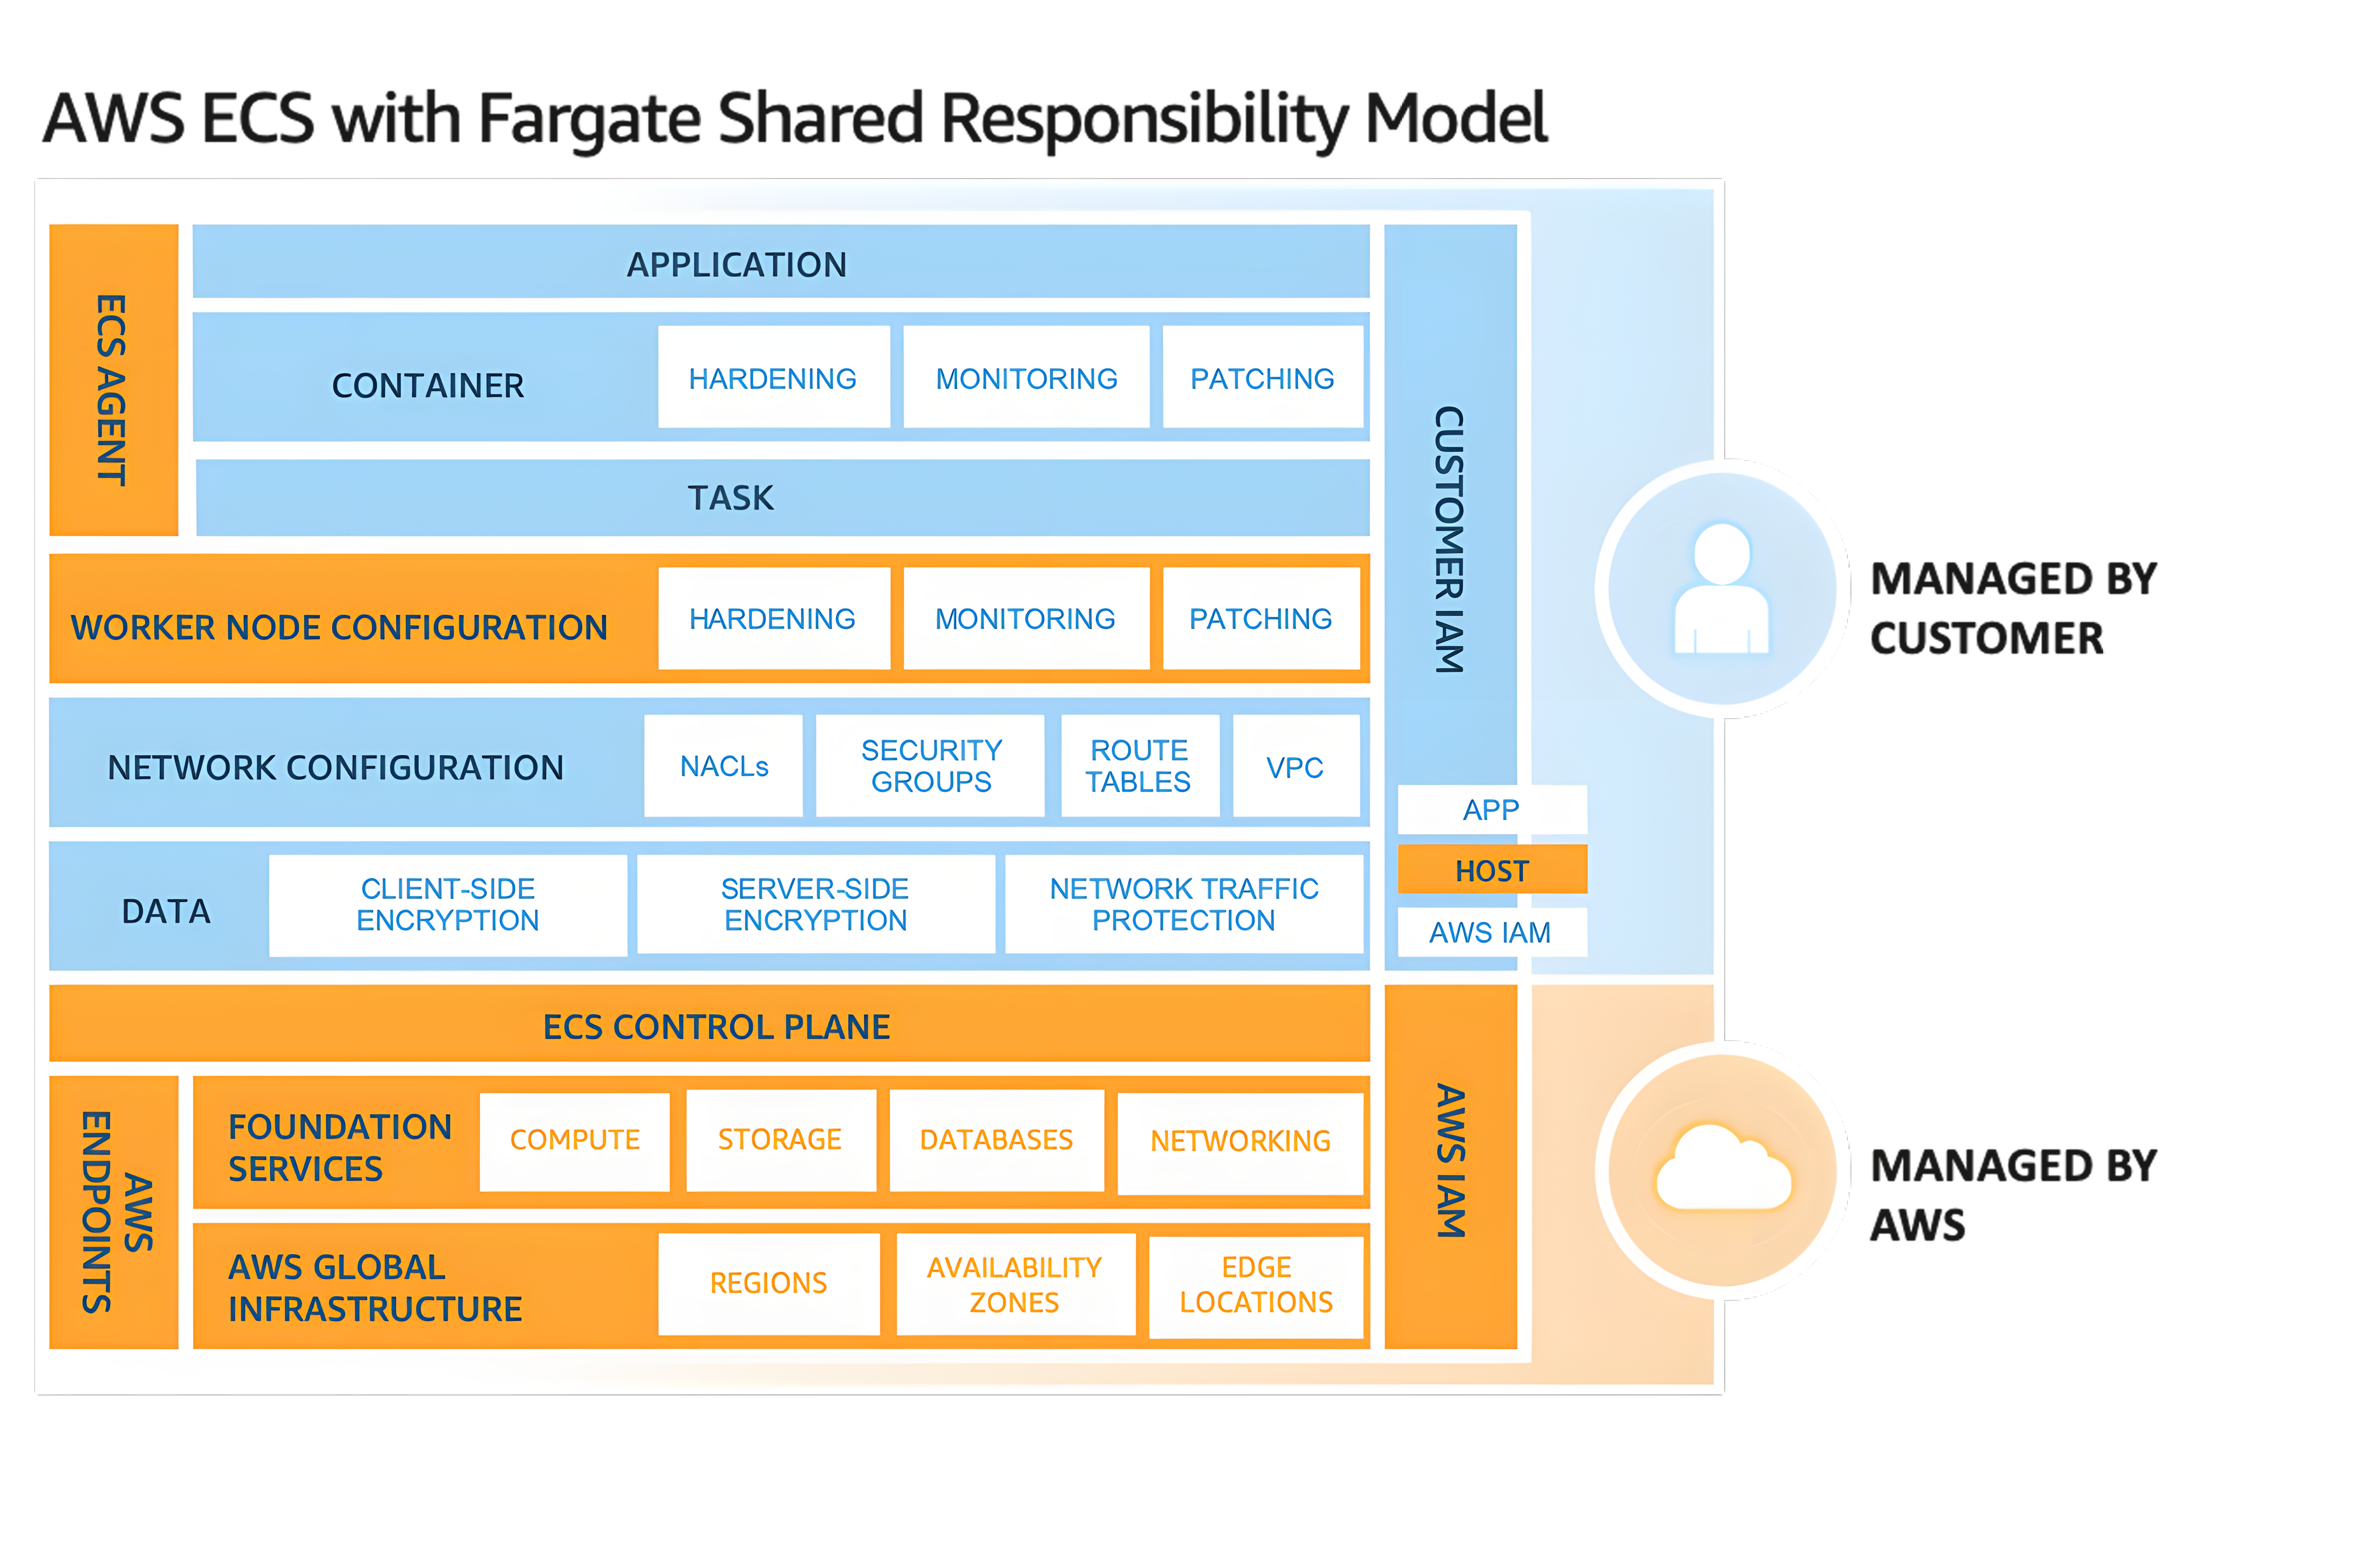
\includegraphics[width=0.9\textwidth]{aws_shared_responsibility_model}
    \caption{Modello di Responsabilità Condivisa di AWS}
    \label{fig:shared_responsibility}
\end{figure}

D'altro canto, il cliente è responsabile della \textit{sicurezza "nel" cloud ("security in the cloud")}. La natura e l'estensione di questa responsabilità dipendono dai servizi AWS scelti e dalla loro astrazione. Ad esempio, per un servizio IaaS come Amazon EC2, il cliente deve gestire la sicurezza del sistema operativo guest (installazione di patch, hardening), di tutte le applicazioni e software installati, e la configurazione dei controlli di rete a livello di istanza (come i Security Group, che agiscono da firewall stateful) e di sottorete (Network ACLs, liste di controllo accessi di rete) \cite{aws-shared-responsibility}. Per servizi più astratti o gestiti, come Amazon S3 (storage) o Amazon DynamoDB (database NoSQL), AWS gestisce l'infrastruttura sottostante, il sistema operativo e la piattaforma applicativa. Tuttavia, spetta al cliente proteggere i dati che carica e le applicazioni che vi accedono: ciò include la corretta configurazione delle policy di accesso (tramite AWS Identity and Access Management - IAM), la cifratura dei dati sensibili (a riposo e in transito, se non gestita nativamente dal servizio per specifici casi d'uso), la gestione delle chiavi di crittografia e l'applicazione di criteri di rete appropriati \cite{aws-shared-responsibility}. In pratica, AWS fornisce gli strumenti e i meccanismi di sicurezza (crittografia, isolamento di rete, logging e auditing, ecc.), ma la loro corretta implementazione, configurazione e la gestione operativa della sicurezza applicativa e dei dati rimangono a carico del cliente.

Per una startup fintech, una profonda e continua comprensione di questo modello è fondamentale: essa guida l'allocazione delle risorse interne dedicate alla sicurezza, la definizione dei processi di compliance (ad esempio, per PCI DSS o GDPR, dove la startup deve dimostrare di aver adempiuto alle proprie responsabilità), la progettazione di controlli di sicurezza specifici per i dati finanziari e le transazioni dei propri clienti, e la corretta configurazione dei servizi AWS per costruire un ambiente sicuro e resiliente. La mancata comprensione di queste responsabilità può portare a vulnerabilità significative e a non conformità normative.